\section{Psoc} \label{sub:sw_impl_psoc_psoc}
\subsection{Psoc}
PSoC'ens formål er at simplificere alt \IIC kommunikation, hvilket viste sig at være en nødvendighed, da implementeringen på Pi'en gav uforudsete problemer med kommunikationen med distancesensorerne.
Da der på Pi'en kører en Linux-distribution foregår \IIC kommunikationen som skrivning og læsning til og fra device-files der repræsenterer de respektive pins (SDA \& SCL), og da kommunikationen med distancesensorerne følger følgende protokollen fra Hardwaredesign afsnittet for distancesensoren.
Ydermere viste det sig at tachometeret, der vha. en schmittrigger trækkes til stel hver gang der detekteres en magnet, dette bliver detekteret som logisk lav på PSoC'en og  kalder den implementerede interrupt service rutine \texttt{ISR}. 
Det vil optage udnødvendig meget af Pi'ens processor og vil være meget tidskritisk i forhold til de andre opgaver som Pi-programmet varetager. Derfor beslutning om at ændre designretning.

Kravet til PSoC'en er, at koden der ligger herpå skal være så hurtig og effektiv som muligt, således at den kan aflæses når PI'en spørger på ny data. 
I listing \ref{lst:getDistance_FL2} ses implementeringen af denne kode.

\lstinputlisting
	[linerange=getDistance::FL-getDistance::FL1, caption=]
	{../../src/psoc/psoc_bil_1/psoc_bil.cydsn/main.c}

\lstinputlisting
	[linerange=getDistance::FL2-getDistance::FL3, label=lst:getDistance_FL2, caption=Front Left sensor aflæsningscyklus.]
	{../../src/psoc/psoc_bil_1/psoc_bil.cydsn/main.c}
	
aflæsningscyklus for de enkelte sensorer er identiske blot med ændret navn og index i \texttt{sendBuffer}

Tachometeret er simplere at aflæse, da alt dataen i forvejen er placeret på PSoC'en. I listing \ref{lst:sw_impl_psoc_getVelocity} ses interrupt service rutinen som køres hver gang der detekteres en magnet på hallswitchen.

\lstinputlisting
	[linerange=getVelocity::1-getVelocity::2, label=lst:sw_impl_psoc_getVelocity, caption=ISR til getVelocity.]
	{../../src/psoc/psoc_bil_1/psoc_bil.cydsn/main.c}

Til sidst kan implementeringen af programmets \texttt{main}-funktion ses i listing \ref{lst:sw_impl_psoc_main}

\lstinputlisting[linerange=main::1-main::2, label=lst:sw_impl_psoc_main, caption=Main program på PSoC.]{../../src/psoc/psoc_bil_1/psoc_bil.cydsn/main.c}

\clearpage

\subsection{Modultest for PSoC}

For at teste om kommunikationen imellem distancesensorene og PSoC'en fungerer korrekt, blev der foretaget en modultest, hvor følgende ønskedes opfyldt. 

\begin{enumerate}
  \item at der kan skrives korrekte kommander til alle 4 sensorer.
  \item at der kan læses korrekte 2-bytes værdier fra alle 4 sensorer.
\end{enumerate}

Der afvikles et main\_test program hvor der kontinuerligt skrives til de 4 sensorer én for én, og derefter læses den nuværende værdi retur i 2-bytes format. 

På figur \ref{fig:write_FL} til \ref{fig:write_RR} ses \texttt{write}-kommando sendt til alle 4 sensorer: 

\begin{figure}[h]
	\centering
	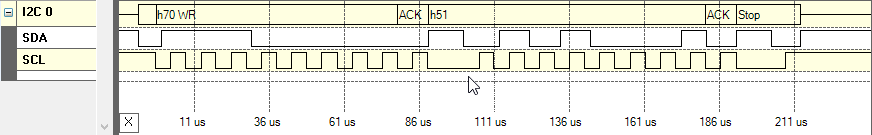
\includegraphics[scale=0.6]{../fig/billeder/psoc_distancesensor_modultest/I2C_write_0x70_FL.png}
	\caption{write til adresse 0x70 sensor FL}
	\label{fig:write_FL}
\end{figure}

\begin{figure}[h]
	\centering
	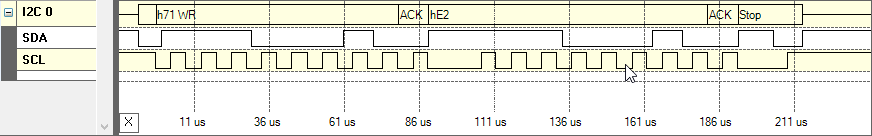
\includegraphics[scale=0.6]{../fig/billeder/psoc_distancesensor_modultest/I2C_write_0x71_FR.png}
	\caption{write til adresse 0x71 sensor FR}
	\label{fig:write_FR}
\end{figure}

\begin{figure}[h]
	\centering
	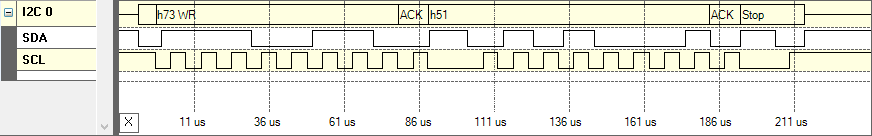
\includegraphics[scale=0.6]{../fig/billeder/psoc_distancesensor_modultest/I2C_write_0x73_RL.png}
	\caption{write til adresse 0x73 sensor RL}
	\label{fig:write_RL}
\end{figure}

\begin{figure}[h]
	\centering
	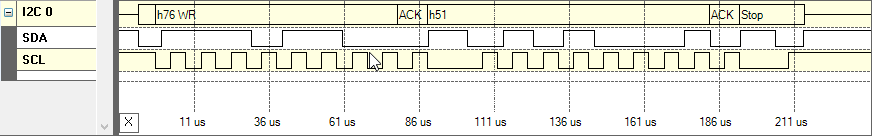
\includegraphics[scale=0.6]{../fig/billeder/psoc_distancesensor_modultest/I2C_write_0x76_RR.png}
	\caption{write til adresse 0x76 sensor RR}
	\label{fig:write_RR}
\end{figure}

\newpage

På figur \ref{fig:read_FL} til \ref{fig:read_RR} ses \texttt{read}-kommando sendt til alle 4 sensorer:

\begin{figure}[h]
	\centering
	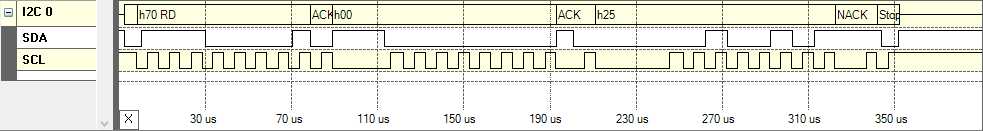
\includegraphics[scale=0.6]{../fig/billeder/psoc_distancesensor_modultest/I2C_read_0x70_FL.png}
	\caption{read til adresse 0x70 sensor FL}
	\label{fig:read_FL}
\end{figure}

\begin{figure}[h]
	\centering
	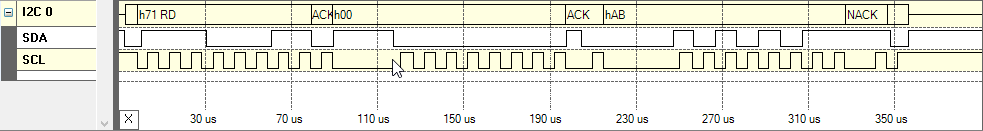
\includegraphics[scale=0.6]{../fig/billeder/psoc_distancesensor_modultest/I2C_read_0x71_FR.png}
	\caption{read til adresse 0x71 sensor FR}
	\label{fig:read_FR}
\end{figure}

\begin{figure}[h]
	\centering
	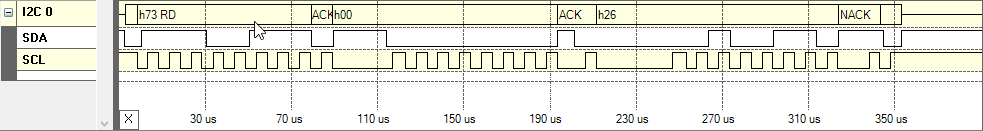
\includegraphics[scale=0.6]{../fig/billeder/psoc_distancesensor_modultest/I2C_read_0x73_RL.png}
	\caption{read til adresse 0x73 sensor RL}
	\label{fig:read_RL}
\end{figure}

\begin{figure}[h]
	\centering
	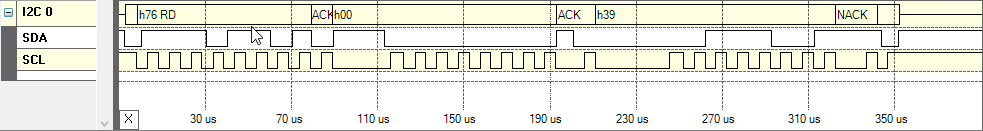
\includegraphics[scale=0.6]{../fig/billeder/psoc_distancesensor_modultest/I2C_read_0x76_RR.png}
	\caption{read til adresse 0x76 sensor RR}
	\label{fig:read_RR}
\end{figure}
